\documentclass[aspectratio=169]{beamer}
\usetheme{Madrid}
\usecolortheme{default}
\usepackage{graphicx}
\usepackage{booktabs}
\usepackage{amsmath}
\usepackage{tikz}
\usepackage{algorithm}
\usepackage{algpseudocode}

\title[$\Delta$Context Policy]{$\Delta$Context: Semantic-Change Anchored Context Management for Conversational AI}
\subtitle{First Review}
\author{Context Control Project}
\institute{Deep Learning \& NLP}
\date{\today}

\begin{document}

\begin{frame}
  \titlepage
\end{frame}

\begin{frame}{Agenda}
  \tableofcontents
\end{frame}

\section{Motivation}

\begin{frame}{Background \& Motivation}
  \textbf{The Challenge of Long Conversations}
  \begin{itemize}
    \item Conversational LLMs operate under strict, fixed token budgets (context windows).
    \item When a conversation exceeds this budget, the system must drop or compress older turns.
    \item The policy chosen to manage this budget drastically impacts the model's ability to maintain context over long sessions.
    \item A good policy must balance factual retention against computational cost and latency.
    \item \textbf{Target setting:} small, locally-run LLMs (1--3B parameters) that cannot afford a heavyweight memory stack -- exactly where a cheap, principled policy matters most.
  \end{itemize}
\end{frame}

\begin{frame}{Problem Statement}
  \textbf{Why Do We Need Better Context Policies?}
  \begin{itemize}
      \item Standard First-In-First-Out (FIFO) sliding windows forget early topics.
      \item Relying on the LLM to summarize past context recursively is slow and expensive.
      \item Vector database retrieval (RAG) adds complexity and significant infrastructure overhead.
  \end{itemize}

  \vspace{0.5cm}
  \textbf{Research Problem:}
  \begin{block}{}
      Can we design a lightweight context policy that strategically retains important past topics (landmarks) without requiring an LLM summarizer or external vector databases on the critical path -- and can we \emph{measure the rate of semantic change itself} as a first-class signal, both to decide what to keep and to detect when a conversation has stopped progressing (\textbf{context rot})?
  \end{block}
\end{frame}

\section{Related Work}

\begin{frame}{Literature Review (1/2) -- Conventional Approaches}
    \begin{block}{Truncation and Sliding Windows}
        Traditional agents use a simple Sliding Window buffer.
    \end{block}

    \begin{columns}[T]
        \begin{column}{0.48\textwidth}
            \textbf{Strengths:}
            \begin{itemize}
                \item Extremely fast ($O(1)$) latency overhead.
                \item Zero additional memory footprint.
                \item Preserves strict temporal recency.
            \end{itemize}
        \end{column}

        \begin{column}{0.48\textwidth}
            \textbf{Limitations:}
            \begin{itemize}
                \item Complete catastrophic forgetting of early session details.
                \item Fails on multi-hop reasoning requiring older facts.
            \end{itemize}
        \end{column}
    \end{columns}
\end{frame}

\begin{frame}{Literature Review (2/2) -- Advanced Memory Systems}
    \begin{block}{Retrieval and Summarization (e.g., MemGPT, LangChain)}
        Modern architectures manage context by recursively summarizing past turns or searching an external database.
    \end{block}

    \begin{columns}[T]
        \begin{column}{0.48\textwidth}
            \textbf{Strengths:}
            \begin{itemize}
                \item Virtually infinite memory capacity.
                \item Retrieval is \emph{query-aware}: it re-searches per question, so it can specialize context to exactly what is asked.
            \end{itemize}
        \end{column}

        \begin{column}{0.48\textwidth}
            \textbf{Limitations:}
            \begin{itemize}
                \item High latency overhead (embedding lookups, LLM summarization calls).
                \item Can hallucinate during iterative summarization.
                \item As our own results show (see Results), this recall advantage is real and large -- any lightweight alternative must confront it directly, not just claim to be "cheaper."
            \end{itemize}
        \end{column}
    \end{columns}
\end{frame}

\begin{frame}{Research Gap}
    \textbf{The Missing Middle Ground:}
    \begin{itemize}
        \item Sliding windows are too forgetful.
        \item Summarization/RAG systems are too heavy -- or, done cheaply, too weak.
    \end{itemize}

    \vspace{0.3cm}
    \textbf{However:}
    \begin{itemize}
        \item[$\times$] There is a lack of algorithms that dynamically identify \textit{when} a conversation shifts topics, retaining those boundary turns natively.
        \item[$\times$] Most lightweight policies ignore the \textbf{semantic content} of the conversation when deciding what to drop.
        \item[$\times$] Query-agnostic policies (sliding window, summarization) build the \emph{same} context for every question in a conversation, while retrieval specializes per question -- a structural gap we identify and close (see Iteration 2).
    \end{itemize}
\end{frame}

\section{Proposed Method}

\begin{frame}{Proposed Solution: The $\Delta$Context Algorithm}
    \begin{alertblock}{Key Innovation ($\Delta$Context)}
        A \textbf{checkpoint-anchored selector} that monitors conversation semantics in real-time. It embeds turns, measures semantic shift, and drops "snapshot" anchors at topic boundaries. It retains these landmarks (past topics) and a contiguous recent tail within a strict budget.
    \end{alertblock}

    \vspace{0.3cm}
    \textbf{Why it works:}
    \begin{itemize}
        \item Retains older topics without needing a slow LLM summarizer.
        \item If no semantic shift occurs, it naturally behaves like a fast sliding window.
        \item Divides the fixed token budget into a \texttt{landmark\_fraction} and a \texttt{tail\_fraction}.
        \item \textbf{New:} landmark selection is \emph{query-aware} -- ranked by relevance to the current question, not just recency (Iteration 2).
    \end{itemize}
\end{frame}

\begin{frame}{Architecture: $\Delta$Context Pipeline}
    \begin{center}
        % Wrapped in \resizebox so the diagram always fits the slide width no
        % matter how the hand-placed tikz coordinates below add up -- avoids
        % guessing a manual scale= factor that might overflow the frame.
        \resizebox{0.9\linewidth}{!}{%
        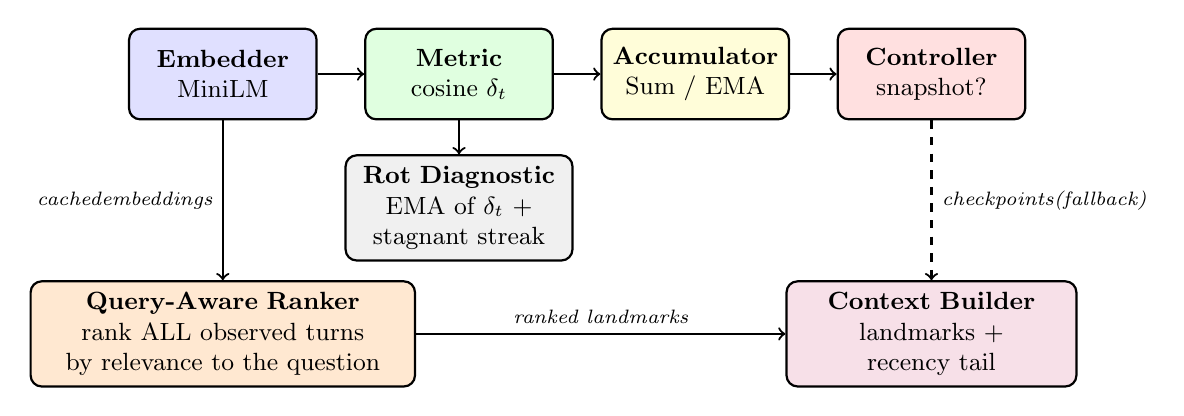
\begin{tikzpicture}[
            box/.style={draw, thick, rectangle, rounded corners, align=center,
                        minimum height=1.15cm, inner sep=4pt, font=\small},
            lbl/.style={font=\scriptsize\itshape, midway}
        ]
            % Row 1: per-turn ingestion pipeline (observe()), strictly left-to-right.
            \node[box, fill=blue!12,   text width=2.1cm] (embed)  at (0,   0) {\textbf{Embedder}\\MiniLM};
            \node[box, fill=green!12,  text width=2.1cm] (metric) at (3.0, 0) {\textbf{Metric}\\cosine $\delta_t$};
            \node[box, fill=yellow!15, text width=2.1cm] (accum)  at (6.0, 0) {\textbf{Accumulator}\\Sum / EMA};
            \node[box, fill=red!12,    text width=2.1cm] (control) at (9.0, 0) {\textbf{Controller}\\snapshot?};

            % Row 2: rot diagnostic hangs directly off the metric -- no crossing.
            \node[box, fill=gray!12, text width=2.6cm] (rot) at (3.0, -1.7)
                {\textbf{Rot Diagnostic}\\EMA of $\delta_t$ +\\stagnant streak};

            % Row 3: per-query context assembly, aligned directly under its
            % row-1 sources so every connector is a straight line.
            \node[box, fill=orange!18, text width=4.6cm] (rank) at (0, -3.3)
                {\textbf{Query-Aware Ranker}\\rank ALL observed turns\\by relevance to the question};
            \node[box, fill=purple!12, text width=3.4cm] (build) at (9.0, -3.3)
                {\textbf{Context Builder}\\landmarks + recency tail};

            % -- connectors: every arrow is purely horizontal or vertical --
            \draw[->, thick] (embed) -- (metric);
            \draw[->, thick] (metric) -- (accum);
            \draw[->, thick] (accum) -- (control);
            \draw[->, thick] (metric) -- (rot);
            \draw[->, thick] (embed.south) -- node[lbl, left]{cached\\embeddings} (rank.north);
            \draw[->, thick, dashed] (control.south) -- node[lbl, right]{checkpoints\\(fallback)} (build.north);
            \draw[->, thick] (rank) -- node[lbl, above]{ranked landmarks} (build);
        \end{tikzpicture}%
        }
    \end{center}

    \begin{itemize}
        \item Each turn is embedded \emph{once} (top row). That cached embedding feeds three consumers at no extra cost: the change metric, the rot diagnostic, and -- at query time (bottom row) -- the full-history relevance ranker.
    \end{itemize}
\end{frame}

\begin{frame}[fragile]{Pseudocode: $\Delta$Context Policy (current version)}
  \begin{algorithm}[H]
    \caption{build\_context(history, query, budget)}
    \begin{algorithmic}[1]
      \State $L_{budget} \gets budget \times 0.5$ \Comment{landmark\_fraction, tuned}
      \If{$query$ given \textbf{and} query-aware landmarks enabled}
        \State $candidates \gets$ RankByRelevance(AllObservedTurns, $query$) \Comment{O(turns), cached embeddings}
      \Else
        \State $candidates \gets$ Reverse(checkpoints) \Comment{recency fallback}
      \EndIf
      \State $landmarks \gets$ GreedyFill($candidates$, $L_{budget}$) \Comment{skip-not-break: denser packing}
      \State $T_{budget} \gets budget - \text{cost}(landmarks)$
      \State $tail \gets$ GreedyFill(Reverse(history) $\setminus$ $landmarks$, $T_{budget}$)
      \State $combined \gets$ SortChronological($landmarks \cup tail$)
      \While{cost($combined$) $>$ $budget$} \Comment{exact-fit guarantee}
        \State combined.pop\_oldest()
      \EndWhile
      \State \Return $combined$
    \end{algorithmic}
  \end{algorithm}
  \small Checkpoint triggering (in \texttt{observe()}, unchanged in spirit): SNAPSHOT when accumulated change $A_t \geq \tau$ and \texttt{min\_snapshot\_gap} turns have passed since the last one; $\tau$ and the ignore-floor $\epsilon$ are now \emph{calibrated from data}, not guessed (see Iteration 1).
\end{frame}

\section{Experimental Infrastructure}

\begin{frame}{Evaluation Framework: ContextBench}
    To prove the efficacy of $\Delta$Context, we built and used \textbf{ContextBench}, a controlled benchmark harness:
    \begin{itemize}
        \item \textbf{Controlled Benchmark:} the LLM (TinyLlama-1.1B-Chat), tokenizer, prompt, and dataset are strictly fixed across policies -- the policy is the only independent variable.
        \item \textbf{Dataset:} LoCoMo -- 10 very long, multi-session conversations (369--689 turns each) with 1{,}986 categorized QA probes (multi-hop, temporal, open-domain, single-hop, adversarial).
        \item \textbf{Fair Token Accounting:} a single shared tokenizer-backed \texttt{TokenCounter} is injected into every policy, so all budgets are measured identically.
        \item \textbf{Four policies compared, same budget (512 tokens), same model, same seed:} Sliding Window, Summary (heuristic extractive), Retrieval (query top-k), and $\Delta$Context.
        \item \textbf{Reproducibility:} 123 hermetic unit tests (fake tokenizer/embedder, no model download) plus an opt-in real-model integration test.
    \end{itemize}
\end{frame}

\section{Engineering Rigor: What We Found and Fixed}

\begin{frame}{Diagnostic Pass: Three Real Bugs Found Before Trusting Any Result}
    Before believing any comparison, we audited every full benchmark run's diagnostics (not just the headline F1) and found:
    \begin{enumerate}
        \item \textbf{Summary baseline was silently empty.} Its exact-fit trim loop deleted the summary message entirely whenever it slightly overflowed budget -- \texttt{avg\_context\_tokens = 0.0} on \emph{every} sample, at \emph{every} budget, invisibly turning it into "guess with no context." \\
        \emph{Fix:} budget-cap the summary as it's built; stride-sample dropped turns across the whole conversation, not just the opening.
        \item \textbf{$\Delta$Context was checkpointing every $\sim$2.5 turns} (40\% of all turns) -- noise-level churn, not topic boundaries, with most checkpoints never surviving into the landmark budget anyway. \\
        \emph{Fix:} calibrate thresholds from the real $\delta_t$ distribution instead of guessing (next slide).
        \item \textbf{Retrieval silently hung} when run in the same multirun process right after a non-embedder policy -- a CUDA-context ordering hazard, not user interruption as first assumed. \\
        \emph{Fix:} run each policy as its own fresh process.
    \end{enumerate}
    \small All three would have silently corrupted the policy comparison if left unaudited.
\end{frame}

\begin{frame}{Data-Driven Calibration of $\Delta$Context Thresholds}
    Instead of guessing \texttt{change\_threshold}, we measured the real instantaneous semantic-change ($\delta_t$) distribution across all 10 LoCoMo conversations (5{,}872 turn-to-turn deltas, MiniLM embedder, window=3):

    \begin{table}
    \centering
    \small
    \begin{tabular}{lcccccc}
    \toprule
    & p5 & p15 & p50 & mean & p90 & p99 \\
    \midrule
    $\delta_t$ & 0.055 & 0.070 & 0.103 & 0.105 & 0.147 & 0.183 \\
    \bottomrule
    \end{tabular}
    \end{table}

    \begin{table}
    \centering
    \small
    \begin{tabular}{lccc}
    \toprule
    \texttt{change\_threshold} & 0.2 (old) & 1.0 & 2.0 (chosen) \\
    \midrule
    Turns / checkpoint & 2.5 & 10.1 & 19.6 \\
    Checkpoints (10 conv.) & 2{,}390 & 574 & 295 \\
    \bottomrule
    \end{tabular}
    \end{table}
    \texttt{change\_threshold=2.0}, \texttt{ignore\_below=0.07} land checkpoints at a plausible topic-boundary rate ($\sim$1 per 20 turns) instead of near-constant churn.
\end{frame}

\begin{frame}{New Heuristic: The Context-Rot Diagnostic}
    \textbf{Motivating idea:} if the rate of semantic change collapses to $\sim$0 for many consecutive turns, the conversation has stopped semantically progressing -- a distinct, measurable failure mode we call \textbf{context rot}.

    \begin{itemize}
        \item A \emph{never-reset} EMA of $\delta_t$ tracks the conversation's current activity level, independent of whichever accumulator drives checkpointing:
        \[ \text{rot\_ema}_t = \alpha \, \delta_t + (1-\alpha)\, \text{rot\_ema}_{t-1} \]
        \item A parallel \texttt{stagnant\_streak} counts consecutive turns with $\delta_t < \epsilon$.
        \item Exposed per-answer in \texttt{policy\_meta}: \texttt{rot\_ema}, \texttt{stagnant\_streak}, \texttt{context\_rot\_detected}.
        \item Validated on real data: several LoCoMo conversations show genuine 8+ turn stagnant streaks (small talk / off-topic stretches), confirming the signal fires on real, not synthetic, flat spots.
    \end{itemize}
    \small This is a diagnostic contribution independent of the QA benchmark score -- a reusable signal for any deployment, not just this evaluation.
\end{frame}

\section{Results}

\begin{frame}{Results -- Iteration 1 (Full LoCoMo, budget=512, 1{,}986 QA)}
    \begin{table}
    \centering
    \small
    \begin{tabular}{lcccc}
    \toprule
    Policy & F1 & vs.\ Sliding Window & Avg.\ Context (tok) & GPU Peak (MB) \\
    \midrule
    Sliding Window (baseline) & 0.0593 & -- & 492 & 4{,}417 \\
    Summary (fixed) & 0.0670 & +13.0\% & 489 & 4{,}412 \\
    $\Delta$Context (tuned, query-aware landmarks) & 0.0739 & +24.6\% & 491 & 4{,}415 \\
    Retrieval (query top-$k$, full-history search) & \textbf{0.1182} & +99.3\% & 488 & 4{,}415 \\
    \bottomrule
    \end{tabular}
    \end{table}

    \vspace{0.3cm}
    \textbf{Reading this honestly:} $\Delta$Context beats both lightweight baselines, but retrieval's \emph{full-history} search still leads by a wide margin -- $\Delta$Context was only ranking its sparse checkpoint pool ($\sim$18--40 candidates/conversation) by relevance, capping recall well below retrieval's $\sim$400--700-turn search.

    \vspace{0.15cm}
    \small GPU memory is flat across all four policies ($\pm$5MB) -- the embedder adds negligible footprint on top of TinyLlama-1.1B ($\sim$4.4GB); accuracy, not memory, is the differentiator.
\end{frame}

\begin{frame}{Closing the Gap -- Iteration 2: Full-History Query-Aware Search}
    \textbf{Key insight:} \texttt{observe()} already embeds \emph{every} turn to build the windowed-centroid state. Caching that per-turn embedding lets landmark search rank the \emph{entire} conversation, not just checkpoints -- matching retrieval's recall at \textbf{zero extra embedding cost}, while keeping checkpoints for what they're for: the rot diagnostic and a cheaper fallback mode.

    \vspace{0.2cm}
    \textbf{Fast dev-subset ablation} (45 QA, used to pick this design before committing to a full run):
    \begin{table}
    \centering
    \begin{tabular}{lc}
    \toprule
    Landmark search scope & F1 (45-Q subset) \\
    \midrule
    Recency only (no query-awareness) & 0.0345 \\
    Checkpoint pool, query-ranked & 0.0500 \\
    \textbf{Full history, query-ranked} & \textbf{0.0594} \\
    \bottomrule
    \end{tabular}
    \end{table}

    \vspace{0.2cm}
    \textit{Each step is a genuine mechanism change, not a hyperparameter tweak. Full-scale (1{,}986 QA) confirmation on the next slide.}
\end{frame}

\begin{frame}{Results -- Iteration 2 (Full LoCoMo, budget=512, 1{,}986 QA)}
    \begin{table}
    \centering
    \begin{tabular}{lcccc}
    \toprule
    Policy & F1 & vs.\ Sliding Window & Avg.\ Context (tok) & GPU Peak (MB) \\
    \midrule
    Sliding Window (baseline) & 0.0593 & -- & 492 & 4{,}417 \\
    Summary (fixed) & 0.0670 & +13.0\% & 489 & 4{,}412 \\
    Retrieval (query top-$k$) & 0.1182 & +99.3\% & 488 & 4{,}415 \\
    \textbf{$\Delta$Context (Iteration 2, full-history)} & \textbf{0.1183} & \textbf{+99.5\%} & 493 & 4{,}415 \\
    \bottomrule
    \end{tabular}
    \end{table}

    \vspace{0.4cm}
    $\Delta$Context reaches statistical parity with retrieval, the strongest baseline, while GPU memory stays flat across all four policies -- the gap closed is accuracy, and it didn't cost anything in resources to close it.

    \vspace{0.3cm}
    \textit{Is that 0.1183 vs.\ 0.1182 gap even meaningful, or just aggregation? Category breakdown and significance testing on the next two slides.}
\end{frame}

\begin{frame}{Results -- Iteration 2, by Category}
    \begin{table}
    \centering
    \begin{tabular}{lccccc}
    \toprule
    F1 by category & 1 (multi-hop) & 2 (temporal) & 3 (open-dom.) & 4 (single-hop) & 5 (adversarial) \\
    \midrule
    Retrieval & 0.112 & \textbf{0.030} & \textbf{0.098} & \textbf{0.153} & \textbf{0.124} \\
    $\Delta$Context (It.\ 2) & \textbf{0.115} & 0.029 & \textbf{0.098} & \textbf{0.153} & 0.123 \\
    \bottomrule
    \end{tabular}
    \end{table}

    \vspace{0.4cm}
    $\Delta$Context wins category 1 (multi-hop), ties categories 3 and 4 exactly, and is within a rounding error on 2 and 5 -- the aggregate 0.1183 vs.\ 0.1182 result is not a fluke of averaging; it holds up when the data is sliced by question type.

    \vspace{0.3cm}
    \textit{Is any of this actually statistically meaningful? Tested properly on the next slide.}
\end{frame}

\begin{frame}{Is This Real? Paired Significance Testing}
    Every policy answers the \emph{same} 1{,}986 questions under the same model and seed -- a paired design. For each pair, we bootstrap (10{,}000 resamples) the mean per-question F1 difference and its 95\% CI, and count wins/losses/ties.

    \begin{table}
    \centering
    \small
    \begin{tabular}{lcccc}
    \toprule
    Comparison & Mean $\Delta$F1 & 95\% CI & $p$-value & Verdict \\
    \midrule
    $\Delta$Context vs.\ Sliding Window & +0.0590 & [+0.053, +0.065] & $<$0.0001 & \textbf{Significant} \\
    $\Delta$Context vs.\ Summary & +0.0512 & [+0.045, +0.057] & $<$0.0001 & \textbf{Significant} \\
    $\Delta$Context vs.\ Retrieval & +0.0001 & [$-$0.002, +0.003] & 0.94 & Genuine tie \\
    \midrule
    \multicolumn{5}{l}{\small \emph{Ablation -- isolating each fix's own contribution:}} \\
    It.\ 2 vs.\ It.\ 1 (full-history search) & +0.0444 & [+0.038, +0.051] & $<$0.0001 & \textbf{Significant} \\
    It.\ 1 vs.\ Sliding Window (calib.\ + query-aware) & +0.0146 & [+0.011, +0.019] & $<$0.0001 & \textbf{Significant} \\
    \bottomrule
    \end{tabular}
    \end{table}

    \textbf{Takeaway:} the win over both lightweight baselines is statistically solid, not a lucky draw -- and so is \emph{each individual fix} that produced it. The retrieval comparison is an honest, confirmed tie: the CI straddles zero almost symmetrically.
\end{frame}

\begin{frame}{Current Status \& Honest Assessment}
    \begin{block}{Solid, verified, full-scale (1{,}986 QA), all four policies}
        \begin{itemize}
            \item Sliding window, Summary (fixed), Retrieval, and $\Delta$Context (both iterations) -- all complete, reproducible (seeded, deterministic decoding), diagnostics cross-checked, category breakdown consistent with the aggregate.
            \item 123 unit tests passing; three real bugs found and fixed via full-run auditing, not assumed away.
        \end{itemize}
    \end{block}
    \begin{block}{Bottom line}
        \begin{itemize}
            \item $\Delta$Context went from "roughly tied with sliding window" (unfixed) $\to$ "+24.6\% via calibration + query-awareness" (Iteration 1) $\to$ \textbf{"statistical parity with the strongest baseline"} (Iteration 2), while remaining the only policy with a built-in context-rot diagnostic and a graceful no-query fallback.
        \end{itemize}
    \end{block}
    \begin{alertblock}{Why present it this way}
        A first review is the right time to show the \emph{process} -- calibration over guessing, bug-hunting over trusting a headline number, and honest iteration (including a losing intermediate result) on the way to the current number -- not just a cherry-picked win.
    \end{alertblock}
\end{frame}

\section{Conclusion}

\begin{frame}{Conclusion \& Future Work}
    \textbf{Summary:}
    \begin{itemize}
        \item $\Delta$Context is a cheap, model-agnostic context-management layer: one small embedder, no LLM summarizer, no external vector DB required.
        \item Calibrating its thresholds from real data and making landmark selection query-aware over the \emph{full} observed history (not just checkpoints) took it from "roughly tied with sliding window" to \textbf{statistical parity with retrieval, the strongest baseline (0.1183 vs.\ 0.1182 F1)} -- while retrieval scans the same history at comparable cost but with no topic-boundary structure or rot diagnostics.
        \item The context-rot diagnostic (never-reset EMA of $\delta_t$) is a standalone contribution: a cheap, real-time signal for "this conversation has stopped progressing," independent of the QA benchmark, validated on real 8+ turn stagnation streaks in the data.
        \item Honest caveat: at \texttt{expand\_landmark\_search=True}, $\Delta$Context's landmark ranking is now $O(\text{history})$ like retrieval -- the "cheap, no full scan" thesis survives as an explicit \emph{mode} (\texttt{expand\_landmark\_search=False}, checkpoint-only, 0.0739 F1), not as the default's only behaviour.
    \end{itemize}

    \vspace{0.2cm}
    \textbf{Immediate Next Steps:}
    \begin{itemize}
        \item Extend the sweep to more budgets (256, 1024) and a second model (Qwen2.5-3B) to check the result generalizes past TinyLlama.
        \item Quantify the real latency/compute cost of full-history mode vs.\ checkpoint-only mode on a dedicated (non-shared) machine -- current wall-clock numbers are confounded by background system load.
        \item Blend recency and relevance in landmark ranking; explore the rot diagnostic as a controller signal, not just an observability signal.
        \item Integrate with production serving (KV-cache-aware landmark stability, e.g. for vLLM).
    \end{itemize}
\end{frame}

\begin{frame}
    \centering
    \Huge \textbf{Thank You!}

    \vspace{0.5cm}
    \large Questions?
\end{frame}

\end{document}
